\documentclass{article}
\usepackage[utf8]{inputenc}
\usepackage{graphicx}
\usepackage{hyperref}
\usepackage{amsmath}
\usepackage[margin=0.5in]{geometry}
\usepackage{mathtools}
\DeclarePairedDelimiter\bra{\langle}{\rvert}
\DeclarePairedDelimiter\ket{\lvert}{\rangle}
\DeclarePairedDelimiterX\braket[2]{\langle}{\rangle}{#1 \delimsize\vert #2}

\begin{document}

\noindent Source code (specific to \texttt{ibmqx2}) from Mark Fingerhuth at \\ \url{https://github.com/markf94/ibmq_code_epl_119_60002}

\noindent copied here on Overleaf. \\

\noindent Note that IBM machine displays qubits in reverse order:
\begin{equation*}
\ket{q_4, q_3, q_2 = \mbox{class}, q_1, q_0 = \mbox{ancilla}}
\end{equation*}

\noindent The algorithm includes a post-selection conditional on the ancilla qubit being~0.  This means we need to discard results where the ancilla is~1 reducing the relevant space to quantum states~$\ket{01110}, \ket{01000}, \ket{00110}, \ket{00000}$.  This creates a normalizing constant:
\begin{equation*}
Z = \mbox{Pr}(\ket{01110}) + \mbox{Pr}(\ket{01000}) + \mbox{Pr}( \ket{00110}) + \mbox{Pr}(\ket{00000})
\end{equation*}

\paragraph{Classification of the input vector $x^\prime$.}

\begin{eqnarray*}
Z &=& 0.267 + 0.417 + 0.007 + 0.036 = 0.727 \\
\mbox{Pr}(\ket{c}=\ket{0}) &=& \frac{\mbox{Pr}(\ket{01000}) + \mbox{Pr}(\ket{00000})}{Z} = \frac{0.417 + 0.036}{Z} = 0.623 \\
\mbox{Pr}(\bra{c}=\bra{1}) &=& \frac{\mbox{Pr}(\ket{01110}) + \mbox{Pr}( \ket{00110})}{Z} = \frac{0.267 + 0.007}{Z} = 0.377
\end{eqnarray*}

\paragraph{Classification of the input vector $x^{\prime \prime} $.}

\begin{eqnarray*}
Z &=& 0.325 + 0.504 + 0.089 + 0 = 0.918 \\
\mbox{Pr}(\ket{c}=\ket{0}) &=& \frac{\mbox{Pr}(\ket{01000}) + \mbox{Pr}(\ket{00000})}{Z} = \frac{0.504 + 0}{Z} = 0.549 \\
\mbox{Pr}(\ket{c}=\ket{1}) &=& \frac{\mbox{Pr}(\ket{01110}) + \mbox{Pr}( \ket{00110})}{Z} = \frac{0.325 + 0.089}{Z} = 0.451
\end{eqnarray*}

\begin{figure}
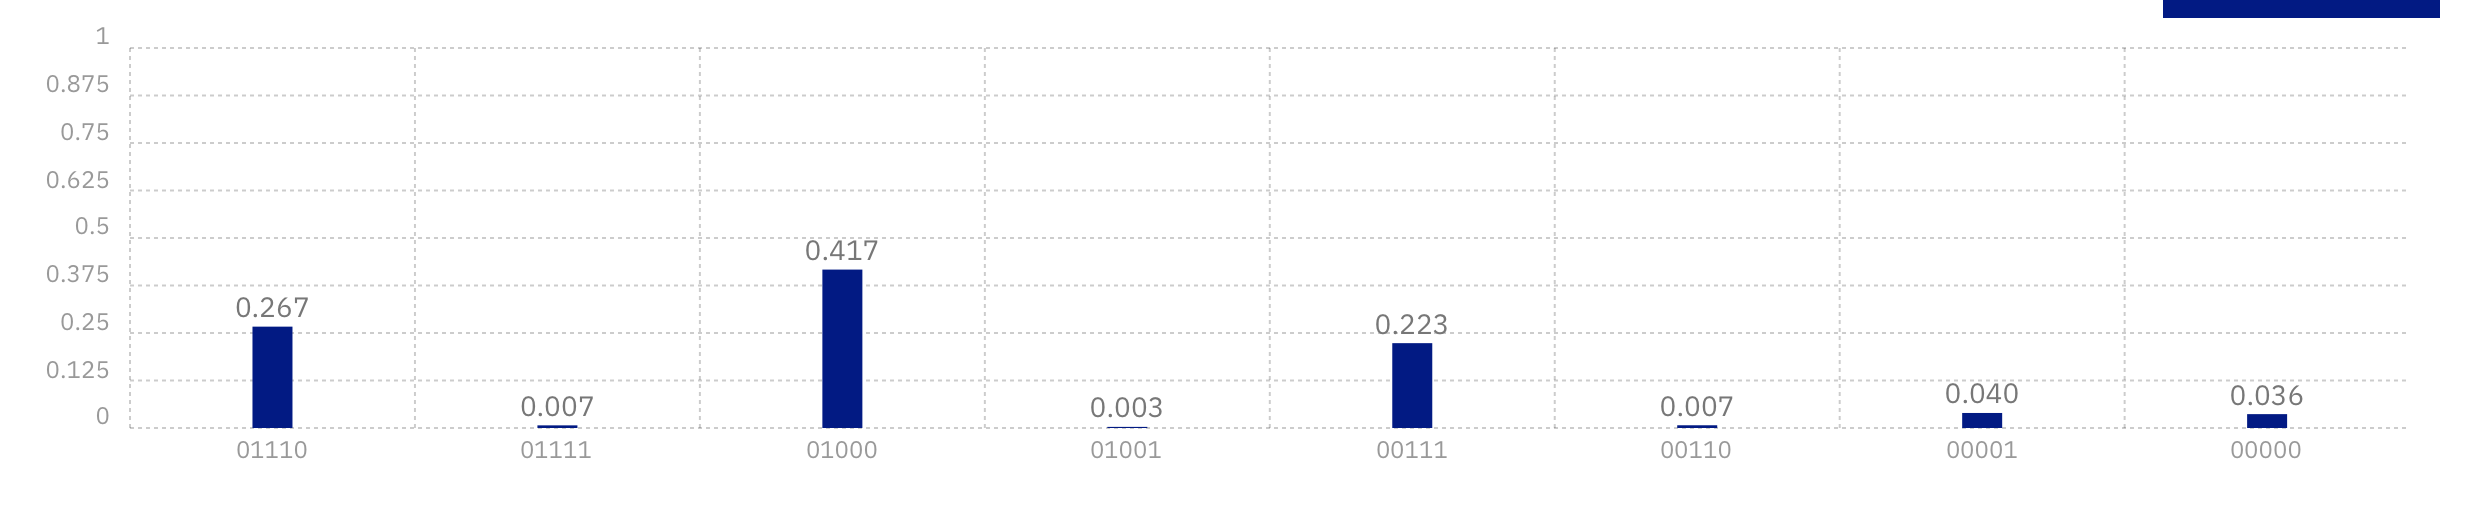
\includegraphics[width=\textwidth]{x0_class0_classification.png}
\centering
\caption{Classification of the input vector $x^\prime$}
\end{figure}

\begin{figure}
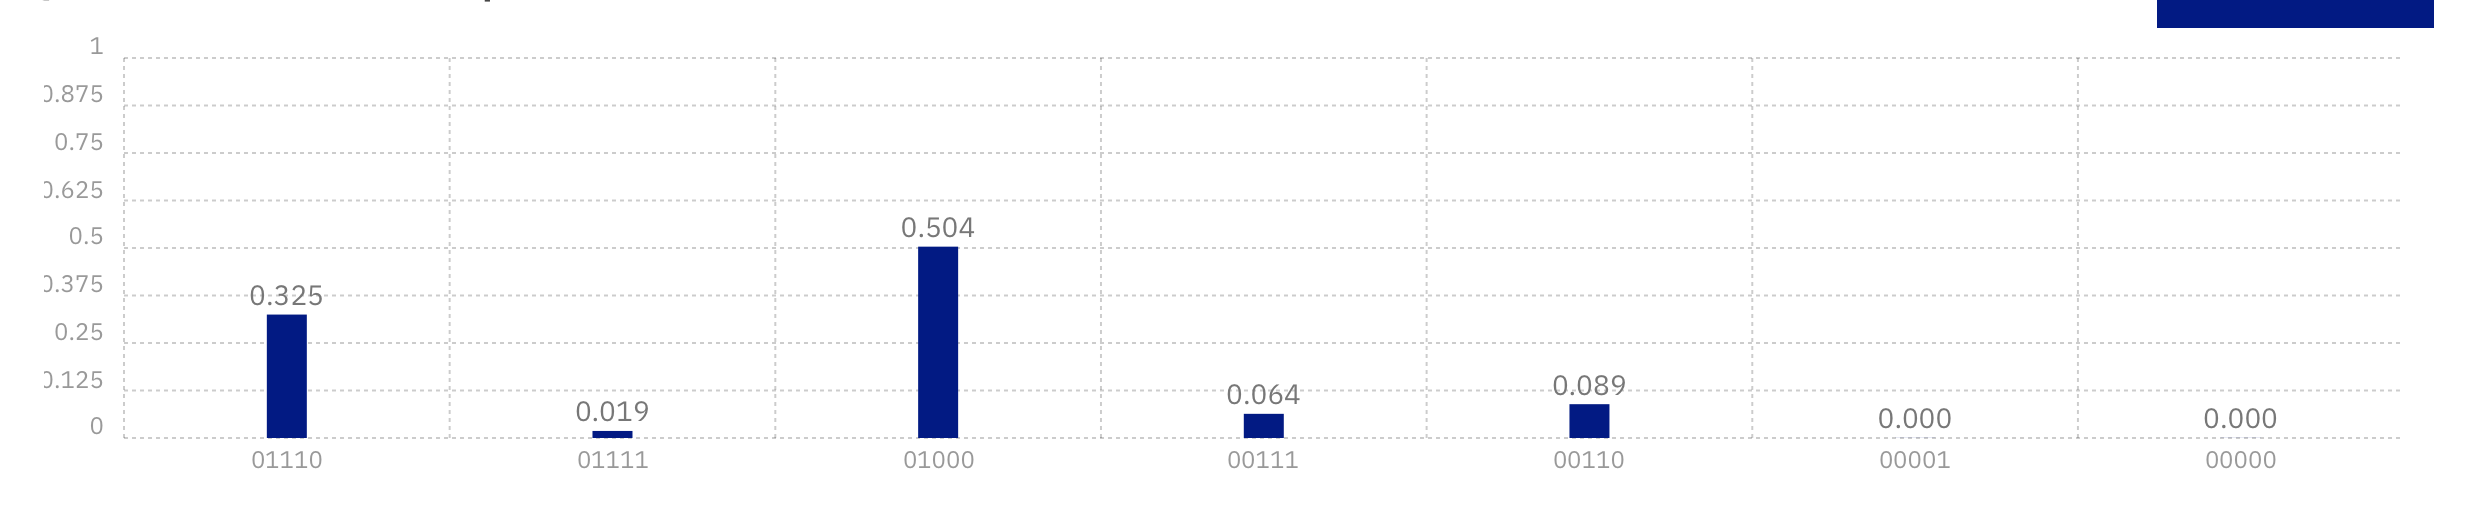
\includegraphics[width=\textwidth]{x1_class0_classification.png}
\centering
\caption{Classification of the input vector $x^{\prime \prime}$}
\end{figure}


\section{Building the quantum circuit}

\noindent The objective of the state preparation is to build the following quantum state:
\begin{equation}
\ket{\mathcal{D}} = \frac{1}{\sqrt{2 M C}} \sum_{m=0}^{M-1} \ket{m}_{\beta} \big( \ket{0}_{\alpha} \ket{\psi_{\bf x^{\prime}}}_{\gamma} + \ket{1}_{\alpha} \ket{\psi_{{\bf x}^m}}_{\gamma} \big) \ket{y^m}_{\delta}
\end{equation}

\noindent containting~$M=2$ training examples and where~$\alpha, \beta, \gamma, \delta$ respectively stand for the ancilla, index, data and class qubits. For clarity and hints about how to actually prepare the state it is useful to expand as:
\begin{equation*}
\ket{\mathcal{D}} = \frac{1}{\sqrt{2 M C}} \big[ \ket{0}_\beta \big( \ket{0}_{\alpha} \ket{\psi_{\bf x^{\prime}}}_{\gamma} + \ket{1}_{\alpha} \ket{\psi_{\bf{x}^0}}_{\gamma} \big) \ket{y^0}_\delta + \ket{1}_\beta \big( \ket{0}_{\alpha} \ket{\psi_{\bf x^{\prime}}}_{\gamma} + \ket{1}_{\alpha} \ket{\psi_{\bf{x}^1}}_{\gamma} \big) \ket{y^1}_\delta  \big]
\end{equation*}

\noindent Vectors to be loaded are:
\begin{eqnarray*}
\ket{\psi_{\bf x^\prime}} &=& -0.549 \ket{0} + 0.836 \ket{1} \\
\ket{\psi_{\bf x^0}} &=&  \ket{1} \\
\ket{\psi_{\bf x^1}} &=&  0.789 \ket{0} + 0.615 \ket{1} \\
\end{eqnarray*}

\noindent The first step consists in bringing the ancilla and the index qubits in a superposition state. This allows to load the first input as entangled with both ancilla and index effectively creating 2 copies of the input vector:
\begin{eqnarray*}
\ket{\mathcal{D}} &=& \ket{0}_\gamma \ket{0}_\beta \ket{0}_\alpha \\
 &\sim& \ket{0}_\gamma \big( \ket{0} + \ket{1} \big)_\beta \big( \ket{0} + \ket{1} \big)_\alpha
\end{eqnarray*}


\noindent The next step is to load the test vector~${\bf x}^{\prime}$.  In this case, we want to entangle the vector only in the case that the ancilla qubit is~$\ket{1}$.
\begin{eqnarray*}
\mbox{CR}_y(\alpha ;\theta, \gamma) &\sim& \ket{0}_\gamma \big( \ket{0} + \ket{1} \big)_\beta \ket{0}_\alpha + \left( \cos \frac{\theta}{2} \ket{0} +	 \sin \frac{\theta}{2}\ket{1} \right)_\gamma \left( \ket{0} + \ket{1} \right)_\beta \ket{1}_\alpha   \\
&\sim&  \ket{0}_\gamma \big( \ket{0} + \ket{1} \big)_\beta \ket{0}_\alpha + \ket{\psi_{\bf x^\prime}}_\gamma \left( \ket{0} + \ket{1} \right)_\beta \ket{1}_\alpha \\
&\sim&  \left( \ket{0} + \ket{1} \right)_\beta \left( \ket{0}_\gamma  \ket{0}_\alpha + \ket{\psi_{\bf x^\prime}}_\gamma \ket{1}_\alpha \right)
\end{eqnarray*}

\noindent where:
\begin{equation*}
\theta \approx 2 \arctan_2(0.835754, -0.549104) \approx 4.304
\end{equation*}

\begin{eqnarray*}
X_\alpha &\sim&  \left( \ket{0} + \ket{1} \right)_\beta \left( \ket{0}_\gamma  \ket{1}_\alpha + \ket{\psi_{\bf x^\prime}}_\gamma \ket{0}_\alpha \right) \\
 &\sim& \ket{0}_\gamma \ket{0}_\beta \ket{1}_\alpha + \ket{0}_\gamma \ket{1}_\beta \ket{1}_\alpha + \left( \ket{0} + \ket{1} \right)_\beta \ket{\psi_{\bf x^\prime}}_\gamma \ket{0}_\alpha  \\
\mbox{Toffoli}(\alpha, \beta ; \gamma) &\sim&  \ket{0}_\gamma \ket{0}_\beta \ket{1}_\alpha + \ket{1}_\gamma \ket{1}_\beta \ket{1}_\alpha + \left( \ket{0} + \ket{1} \right)_\beta \ket{\psi_{\bf x^\prime}}_\gamma \ket{0}_\alpha \\
&\sim&  \ket{0}_\gamma \ket{0}_\beta \ket{1}_\alpha + \ket{\psi_{\bf x^0}}_\gamma \ket{1}_\beta \ket{1}_\alpha + \left( \ket{0} + \ket{1} \right)_\beta \ket{\psi_{\bf x^\prime}}_\gamma \ket{0}_\alpha \\
X_\beta \, \mbox{cute trick...} &\sim&  \ket{0}_\gamma \ket{1}_\beta \ket{1}_\alpha + \ket{\psi_{\bf x^0}}_\gamma \ket{0}_\beta \ket{1}_\alpha + \left( \ket{0} + \ket{1} \right)_\beta \ket{\psi_{\bf x^\prime}}_\gamma \ket{0}_\alpha
\end{eqnarray*}



\noindent The trick moves the first training vector~$\ket{\psi_{\bf x^0}}$ to the~$\ket{0}$ state of the index qubit~$\beta$.  This allows us to now apply another Toffoli gate to load the second vector into the~$\ket{1}$ state of the index and doesn't change anything on the test vector~$\ket{\psi_{\bf x}^\prime}$ since it is already entangled with a index qubit~$\beta$ that is in a superposition state.

\begin{eqnarray*}
X_\beta \, \mbox{cute trick...} &\sim&  \ket{0}_\gamma \ket{1}_\beta \ket{1}_\alpha + \ket{\psi_{\bf x^0}}_\gamma \ket{0}_\beta \ket{1}_\alpha + \left( \ket{0} + \ket{1} \right)_\beta \ket{\psi_{\bf x^\prime}}_\gamma \ket{0}_\alpha \\
&\sim&  \ket{0}_\gamma \ket{1}_\beta \ket{1}_\alpha + \ket{\psi_{\bf x^0}}_\gamma \ket{0}_\beta \ket{1}_\alpha + \ket{\psi_{\bf x}^\prime}_\gamma \ket{0}_\beta \ket{0}_\alpha + \ket{\psi_{\bf x}^\prime}_\gamma \ket{1}_\beta \ket{0}_\alpha \\
\mbox{Toffoli}(\alpha, \beta ; \gamma)  &\sim&  \ket{1}_\gamma \ket{1}_\beta \ket{1}_\alpha + \ket{\psi_{\bf x^0}}_\gamma \ket{0}_\beta \ket{1}_\alpha + \ket{\psi_{\bf x^\prime}}_\gamma \ket{0}_\beta \ket{0}_\alpha + \ket{\psi_{\bf x^\prime}}_\gamma \ket{1}_\beta \ket{0}_\alpha \\
\mbox{CR}_y (\beta ; - \theta, \gamma)  &\sim& \left( R_y(- \theta) \ket{ 1} \right)_\gamma \ket{1}_\beta \ket{1}_\alpha + \ket{\psi_{\bf x^0}}_\gamma \ket{0}_\beta \ket{1}_\alpha + \ket{\psi_{\bf x^\prime}}_\gamma \ket{0}_\beta \ket{0}_\alpha +  \left( R_y(- \theta) \ket{\psi_{\bf x^\prime}} \right)_\gamma \ket{1}_\beta \ket{0}_\alpha \\
\mbox{Toffoli} (\alpha, \beta ; \gamma)  &\sim& \left( \cos \frac{\theta}{2} \ket{0} + \sin \frac{\theta}{2} \ket{1} \right)_\gamma \ket{1}_\beta \ket{1}_\alpha + \ket{\psi_{\bf x^0}}_\gamma \ket{0}_\beta \ket{1}_\alpha + \ket{\psi_{\bf x^\prime}}_\gamma \ket{0}_\beta \ket{0}_\alpha +  \left( R_y(\theta) \ket{\psi_{\bf x^\prime}} \right)_\gamma \ket{1}_\beta \ket{0}_\alpha
\end{eqnarray*}

\noindent The trick above is that~$\left( R_y(- \theta) \ket{\psi_{\bf x^\prime}} \right)_\gamma \ket{1}_\beta \ket{0}_\alpha$ is unaffected by the second Toffoli gate since the ancilla is in state~$\ket{0}$.
\begin{eqnarray*}
\mbox{CR}_y (\beta ; \theta , \gamma)  &\sim& \left[ R_y(\theta) \left(  \cos \frac{\theta}{2} \ket{0} + \sin \frac{\theta}{2} \ket{1} \right) \right]_\gamma \ket{1}_\beta \ket{1}_\alpha + \ket{\psi_{\bf x^0}}_\gamma \ket{0}_\beta \ket{1}_\alpha + \ket{\psi_{\bf x^\prime}}_\gamma \ket{0}_\beta \ket{0}_\alpha +  \left( R_y(\theta) R_y(-\theta) \ket{\psi_{\bf x^\prime}} \right)_\gamma \ket{1}_\beta \ket{0}_\alpha \\
 &\sim& \left( \cos \theta \ket{0} + \sin \theta \ket{1} \right)_\gamma \ket{1}_\beta \ket{1}_\alpha + \ket{\psi_{\bf x^0}}_\gamma \ket{0}_\beta \ket{1}_\alpha + \ket{\psi_{\bf x^\prime}}_\gamma \ket{0}_\beta \ket{0}_\alpha +  \left( \ket{\psi_{\bf x^\prime}} \right)_\gamma \ket{1}_\beta \ket{0}_\alpha \\
  &\sim& \ket{\psi_{\bf x^1}}_\gamma \ket{1}_\beta \ket{1}_\alpha + \ket{\psi_{\bf x^0}}_\gamma \ket{0}_\beta \ket{1}_\alpha + \ket{\psi_{\bf x^\prime}}_\gamma \ket{0}_\beta \ket{0}_\alpha + \ket{\psi_{\bf x^\prime}}_\gamma \ket{1}_\beta \ket{0}_\alpha
\end{eqnarray*}

\noindent where:
\begin{equation*}
\theta \approx \arctan_2(0.61489, 0.78861) \approx 0.662
\end{equation*}

\noindent We are now in a position to introduce the class qubit~$\delta$.  We should simply condition it to be in state~$\ket{1}$ when the index qubit~$\beta$ is also in state~$\ket{1}$ and to leave it to~$\ket{0}$ otherwise.
\begin{eqnarray*}
  &\sim& \big( \ket{\psi_{\bf x^1}}_\gamma \ket{1}_\beta \ket{1}_\alpha + \ket{\psi_{\bf x^0}}_\gamma \ket{0}_\beta \ket{1}_\alpha + \ket{\psi_{\bf x^\prime}}_\gamma \ket{0}_\beta \ket{0}_\alpha + \ket{\psi_{\bf x^\prime}}_\gamma \ket{1}_\beta \ket{0}_\alpha \big) \ket{0}_\delta \\
\mbox{CX}(\delta ; \beta) &\sim&  \big( \ket{\psi_{\bf x^0}}_\gamma \ket{0}_\beta \ket{1}_\alpha + \ket{\psi_{\bf x^\prime}}_\gamma \ket{0}_\beta \ket{0}_\alpha \big) \ket{0}_\delta + \big( \ket{\psi_{\bf x^1}}_\gamma \ket{1}_\beta \ket{1}_\alpha + \ket{\psi_{\bf x^\prime}}_\gamma \ket{1}_\beta \ket{0}_\alpha \big) \ket{1}_\delta \\
&\sim&  \ket{0}_\beta \big(  \ket{\psi_{\bf x^\prime}}_\gamma \ket{0}_\alpha  + \ket{\psi_{\bf x^0}}_\gamma  \ket{1}_\alpha \big) \ket{0}_\delta + \ket{1}_\beta \big(  \ket{\psi_{\bf x^\prime}}_\gamma \ket{0}_\alpha  + \ket{\psi_{\bf x^1}}_\gamma \ket{1}_\alpha \big) \ket{1}_\delta \\
&=& \frac{1}{\sqrt{2 M}} \left( \ket{0}_\beta \big(  \ket{\psi_{\bf x^\prime}}_\gamma \ket{0}_\alpha  + \ket{\psi_{\bf x^0}}_\gamma  \ket{1}_\alpha \big) \ket{0}_\delta + \ket{1}_\beta \big(  \ket{\psi_{\bf x^\prime}}_\gamma \ket{0}_\alpha  + \ket{\psi_{\bf x^1}}_\gamma \ket{1}_\alpha \big) \ket{1}_\delta \right)
\end{eqnarray*}

\noindent Now that the state has been prepared we can finally run the algorithm which consists in applying a single Hadamard gate to the ancilla qubit.
\begin{eqnarray*}
H(\alpha) &=& \frac{1}{2 \sqrt{M}} \left( \ket{0}_\beta \big(  \ket{\psi_{{\bf x^\prime} + {\bf x^0} } }_\gamma \ket{0}_\alpha  + \ket{\psi_{{\bf x^\prime} - {\bf x^0}}}_\gamma  \ket{1}_\alpha \big) \ket{0}_\delta + \ket{1}_\beta \big( \ket{\psi_{{\bf x^\prime} + {\bf x^1}}}_\gamma \ket{0}_\alpha  + \ket{\psi_{ {\bf x^\prime} - {\bf x^1} }}_\gamma \ket{1}_\alpha \big) \ket{1}_\delta \right)  \\
&=& \frac{1}{2 \sqrt{M}} \sum_{m=0}^{M-1} \ket{m}_{\beta} \big( \ket{0}_{\alpha} \ket{\psi_{ {\bf x^\prime} + {\bf x}^m  }}_{\gamma} + \ket{1}_{\alpha} \ket{\psi_{ {\bf x^\prime} - {\bf x}^m}  }_{\gamma} \big) \ket{y^m}_{\delta}
\end{eqnarray*}

\noindent where~$\ket{\psi_{ {\bf x^\prime} \pm {\bf x}^m }} = \ket{\psi_{ {\bf x}^\prime  }} \pm \ket{\psi_{ {\bf x}^m  }} $.  Now we can perform a conditional measurement based on the value of the ancilla qubit:
\begin{eqnarray*}
\mbox{Pr} (\ket{\alpha} = \ket{0}_\alpha) &=& \frac{1}{4M} \left( \vert {\bf x}^\prime + {\bf x^0} \vert^2 + \vert {\bf x}^\prime + {\bf x^1} \vert^2  \right) \\
\mbox{Pr} (\ket{\alpha} = \ket{1}_\alpha) &=& \frac{1}{4M} \left( \vert {\bf x}^\prime - {\bf x^0} \vert^2 + \vert {\bf x}^\prime - {\bf x^1} \vert^2  \right)
\end{eqnarray*}

\noindent TODO:  Maybe remove completely the notation~$\ket{\psi_{\bf x}}_\gamma$ to simply~$\ket{{\bf x}}_\gamma = {\bf x}_0 \ket{0}_\gamma + {\bf x}_1 \ket{1}_\gamma$.  It would also help explain better the final superposition with Hadamard gate. \\

\noindent Therefore if the ancilla is measured~$\ket{\alpha} = \ket{0}$, the post-measurement quantum state is now given by:
\begin{equation}
\ket{\mathcal{D}}_{\ket{\alpha} = \ket{0}_\alpha} = \frac{1}{2 \sqrt{M \mbox{Pr} (\ket{\alpha} = \ket{0}_\alpha) }} \sum_{m=0}^{N-1} \ket{m}_\beta \ket{{\bf x}^\prime + {\bf x}^m }_\gamma \ket{y^m}_\delta
\end{equation}

\noindent This normalized state can be viewed as a weighted sum:
\begin{eqnarray*}
1 &=& \frac{1}{4 M p_{\text{acc}}} \sum_m | {\bf x}^\prime + {\bf x}^m |^2  \\
1 &=& \frac{1}{M p_{\text{acc}}} \sum_m \left( 1 - \frac{1}{4} | {\bf x}^\prime - {\bf x}^m |^2 \right) \\
1 &=& \underbrace{\frac{1}{M p_{\text{acc}}} \sum_{m|y^m=0} \left( 1 - \frac{1}{4} | {\bf x}^\prime - {\bf x}^m |^2 \right)}_{\text{Pr}(\tilde{y} = 0)} + \underbrace{\frac{1}{M p_{\text{acc}}} \sum_{m|y^m=1} \left( 1 - \frac{1}{4} | {\bf x}^\prime - {\bf x}^m |^2 \right)}_{\text{Pr}(\tilde{y} = 1)}
\end{eqnarray*}

\noindent where:
\begin{equation}
\text{Pr}(\tilde{y} = 0) = \frac{1}{4 M p_{\text{acc}}} \sum_{m|y^m=0} \left( 1 - \frac{1}{4} | {\bf x}^\prime + {\bf x}^m |^2 \right)
\label{eq:confidenceClassifier}
\end{equation}

\noindent Clearly, if the more the input vector is ``closer'' to the training input labeled as belonging to class~0, the more the value of~$\text{Pr}(\tilde{y} = 0)$ rises.  Because of the normalization of the post-measurement quantum state above, it is clear that if we find~$\text{Pr}(\tilde{y} = 0) > 0.5$, the prediction is~$0$ otherwise we should predict class~$1$.  This is achieving exactly the same effect as the original classifier.  Running the quantum circuit gives us an experimental value for~$\text{Pr}(\tilde{y} = 0)$ and the LHS gives us confirmation that this value indeed corresponds to the classification task we defined originally.

%\noindent Following identity which is easy to prove for normalized vectors:
%\begin{equation}
%\frac{1}{4} |{\bf x}^\prime + {\bf x}^m|^2 = 1 - \frac{1}{4} | {\bf x}^\prime - {\bf x}^m |^2
%\label{eq:normalizingId}
%\end{equation}


%\newpage
%\section{Question to Maria}

%\noindent After state preparation and conditional measurement on the ancilla being~$\ket{0}$, the state is given by:
%\begin{equation}
%\frac{1}{2\sqrt{M \rho_{\mbox{\tiny acc0}}}} \sum_{m=1}^M \sum_{i=1}^N \ket{m} ( \tilde{x}_i + \tilde{x}_i^m ) \ket{i} \ket{y^m}
%\end{equation}

%\noindent which is normalized to~1 because of the definion of~$\rho_{\mbox{\tiny acc0}}$.  For the sake of simplicity, let's specialize this to 2 training vectors as in the paper where~$x_0$ (resp.~$x_1$) belongs to class~$y=0$ (resp.~$y=1$), we get:
%\begin{equation}
%\frac{1}{4M\rho_{\mbox{\tiny acc0}}} \left( \underbrace{\vert \tilde{x} + x_0 \vert^2}_{\sim \text{Pr}(y=0)} + \underbrace{\vert \tilde{x} + x_1 \vert^2}_{\sim \text{Pr}(y=1)} \right) = 1
%\end{equation}

%\noindent I understand that the goal now is to find the relative importance of~$\text{Pr}(y=0)$ vs.~$\text{Pr}(y=1)$.  Let's assume that:
%\begin{equation}
%\vert \tilde{x} + x_0 \vert^2 \gg \vert \tilde{x} + x_1 \vert^2
%\end{equation}

%\noindent This means that we are going to predict that class~$y=0$ is more probable than~$y=1$ with $\text{Pr}(y=0) \gg \text{Pr}(y=1)$.  \\

%\noindent My issue is that I don't see how this implies:
%\begin{equation}
%\vert \tilde{x} - x_0\vert^2 \ll \vert \tilde{x} - x_1\vert^2  \,\, \text{???}
%\label{eq:question}
%\end{equation}

%\noindent meaning that~$\tilde{x}$ is much closer to~$x_0$ than~$x_1$ which is what we actually care about. I understand that because of the normalization, 
%\begin{equation}
%\underbrace{\frac{1}{4M} \left( |\tilde{x} + x_0|^2 + |\tilde{x} + x_1|^2 \right)}_{\text{Pr(ancilla=0)} = \rho_{\text{acc0}}} = 1 - \underbrace{\frac{1}{4M} \left( |\tilde{x} - x_0|^2 + |\tilde{x} - x_1|^2 \right)}_{\text{Pr(ancilla=1)} = \rho_{\text{acc1}}}
%\end{equation}

%\noindent but somehow, I can't manage to formally get to something like~\ref{eq:question}. \\

%\paragraph{Alternative formulation} In fact, I was wondering why not consider the conditional measurement on the ancilla being~$\ket{1}$ instead of~$\ket{0}$ as presented in the paper.  In this case, we would also have:
%\begin{equation}
%\frac{1}{4M\rho_{\mbox{\tiny acc1}}} \left( \vert \tilde{x} - x_0 \vert^2 + \vert \tilde{x} - x_1 \vert^2 \right) = 1
%\end{equation}

%\noindent In this case, if we are in a situation where:
%\begin{equation}
%\vert \tilde{x} - x_0 \vert^2 \ll \vert \tilde{x} - x_1 \vert^2
%\end{equation}

%\noindent then, it would be quite straightforward to predict class~$y=0$ as the most probable outcome.  Namely, the class with the lowest weight would be the prediction of the algorithm (kind of like the~$1-\text{Pr}$) when the ancilla is measured as~$\ket{0}$ as you do but I don't see the connection...


\end{document}
